
When a multi-strand thermal quench problem is analysed, a quenched zone belonging to one winding heats up the neighbouring ones across the insulation layer. As shown in Fig.~\ref{fig: quench_propagation_heat_flux} the heat flux $\vec{\phi_\text{q}}$ is directed towards the non-quenched neighbouring windings placed outside of a~red, dashed circumference. Therefore, in order to account for the transverse quench propagation, it is required to create an algorithm that detects the temperature above the~critical temperature, $T_\text{c}$ in windings where the~quench has not occurred, yet. In detail, the~algorithm detects quenches and initiates a new quench front propagation when the~temperature outside of the~quenched zone exceeds the~critical temperature of a superconductor. In other words, it is responsible for a turn-to-turn propagation across the~insulation layer between different windings.

\begin{figure}[H]
    \centering
    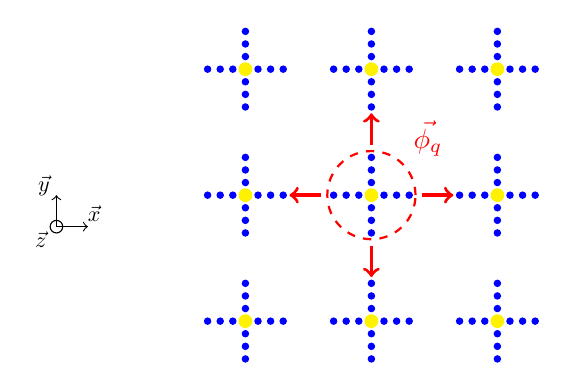
\begin{tikzpicture}[scale = 0.8]
        
        % row number 1  
        \foreach \x in {-3,-2,...,3}
            \filldraw[blue] (\x/5, 0) circle (0.05);
        \foreach \y in {-3,-2,...,3}
            \filldraw[blue] (0, \y/5) circle (0.05);    
         \foreach \x in {-3,-2,...,3}
            \filldraw[blue] (\x/5+2, 0) circle (0.05);
        \foreach \y in {-3,-2,...,3}
            \filldraw[blue] (2, \y/5) circle (0.05);   
        \foreach \x in {-3,-2,...,3}
            \filldraw[blue] (\x/5+4, 0) circle (0.05);
        \foreach \y in {-3,-2,...,3}
            \filldraw[blue] (4, \y/5) circle (0.05);   
        
        % row number 2
        \foreach \x in {-3,-2,...,3}
            \filldraw[blue] (\x/5, 2) circle (0.05);
        \foreach \y in {-3,-2,...,3}
            \filldraw[blue] (0, \y/5+2) circle (0.05);    
         \foreach \x in {-3,-2,...,3}
            \filldraw[blue] (\x/5+2, 2) circle (0.05);
        \foreach \y in {-3,-2,...,3}
            \filldraw[blue] (2, \y/5+2) circle (0.05);   
        \foreach \x in {-3,-2,...,3}
            \filldraw[blue] (\x/5+4, 2) circle (0.05);
        \foreach \y in {-3,-2,...,3}
            \filldraw[blue] (4, \y/5+2) circle (0.05);   
        
        % row number 3
        \foreach \x in {-3,-2,...,3}
            \filldraw[blue] (\x/5, 4) circle (0.05);
        \foreach \y in {-3,-2,...,3}
            \filldraw[blue] (0, \y/5+4) circle (0.05);    
         \foreach \x in {-3,-2,...,3}
            \filldraw[blue] (\x/5+2, 4) circle (0.05);
        \foreach \y in {-3,-2,...,3}
            \filldraw[blue] (2, \y/5+4) circle (0.05);   
        \foreach \x in {-3,-2,...,3}
            \filldraw[blue] (\x/5+4, 4) circle (0.05);
        \foreach \y in {-3,-2,...,3}
            \filldraw[blue] (4, \y/5+4) circle (0.05);   
        \foreach \x in {0,2,4} 
            \foreach \y in {0,2,4} 
                \filldraw[yellow] (\x, \y) circle (0.1);
    
        \draw[thick, red, dashed] (2,2) circle (0.7cm);
        \draw[very thick, red, ->] (2,2.8) -- (2,3.3);
        \draw[very thick, red, ->] (2,1.2) -- (2,0.7);
        \draw[very thick, red, ->] (2.8, 2) -- (3.3,2);
        \draw[very thick, red, ->] (1.2,2) -- (0.7,2);
        \node[red, scale=1] at (2.9,2.9) {$\vec{\phi_\text{q}}$};
        \draw[scale=1] (-3.5+0.5,1+0.5) circle (0.1cm);
        \draw[black, ->, scale=1] (-3.5+0.5,1+0.5) -- (-3.5+0.5,1.5+0.5);
        \draw[black, ->, scale=1] (-3.5+0.5,1+0.5) -- (-3+0.5,1+0.5);
        \node[scale = 0.8] at (-3.75+0.5,0.8+0.5) {$\vec{z}$};
        \node[scale = 0.8] at (-2.9+0.5,1.2+0.5) {$\vec{x}$};
        \node[scale = 0.8] at (-3.7+0.5,1.65+0.5) {$\vec{y}$};
        
    \end{tikzpicture}
    \caption{Heat flux direction from the quenched winding marked in the red circle.}
    \label{fig: quench_propagation_heat_flux}
\end{figure}

Provided that searching starts at node $N$, winding number is $W$, magnetic field strength of the winding $W$ is $B_W$, node temperature is $T_N$ and critical temperature of related winding is $T_{\text{c},}$, the problem is solved as described in Algorithm \ref{alg:quench_detection}.

\begin{algorithm}[H]
    \caption{Quench Detection.}
    \label{alg:quench_detection}
    \begin{algorithmic}[1]
    \STATE \textbf{for} $N$ not quenched \textbf{do}
    \STATE \hspace{0.5cm} check the winding $W$ which node $N$ belongs to
    \STATE \hspace{0.5cm} assign magnetic field $B_W$ of the winding $W$
    \STATE \hspace{0.5cm} calculate $T_{\text{c},W}$ for the magnetic field $B_W$
    \STATE \hspace{0.5cm} \textbf{if} $T(N) > T_{\text{c},}$
    \STATE \hspace{1.0cm} assign node $N$ to a list of newly quenched nodes
    \end{algorithmic}
\end{algorithm}